\documentclass[11pt,a4paper]{article}

\usepackage[margin=1in]{geometry}
\usepackage{graphicx}
\usepackage{booktabs}
\usepackage{longtable}
\usepackage{array}
\usepackage{xcolor}
\usepackage{hyperref}
\usepackage{fancyhdr}
\usepackage{titlesec}
\usepackage{enumitem}
\usepackage{caption}
\usepackage{float}

\hypersetup{
  colorlinks=true,
  linkcolor=blue!45!black,
  urlcolor=blue!45!black,
  citecolor=blue!45!black
}

\pagestyle{fancy}
\fancyhf{}
\lhead{Voice Agent Latency and Reliability Observatory}
\rhead{\thepage}
\setlength{\headheight}{14pt}
\titleformat{\section}{\Large\bfseries}{\thesection}{0.8em}{}
\titleformat{\subsection}{\large\bfseries}{\thesubsection}{0.8em}{}
\setlist[itemize]{leftmargin=1.4em}
\setlist[enumerate]{leftmargin=1.6em}

\newcommand{\statuspass}{\textbf{PASS}}
\newcommand{\statuspartial}{\textbf{PARTIAL}}
\newcommand{\na}{\textit{Not available in the captured benchmark run.}}

\begin{document}

\begin{titlepage}
  \centering
  \vspace*{1.0cm}
  {\Huge \textbf{Voice Agent Latency \& Reliability Observatory}\par}
  \vspace{0.5cm}
  {\Large Benchmarking, Latency Measurement, Model Comparison and Observability for AI Voice Pipelines\par}
  \vspace{1.5cm}
  {\large Author: ValikalaChandra\par}
  \vspace{0.2cm}
  {\large Institution: Not documented in the repository\par}
  \vspace{0.2cm}
  {\large Date: September 2026\par}
  \vfill
  \begin{minipage}{0.85\textwidth}
  \small
  This report summarizes the final repository state. It is based on the checked-in
  implementation, stored benchmark artifacts, screenshots, audit reports, and
  test documentation. It does not invent missing measurements.
  \end{minipage}
\end{titlepage}

\tableofcontents
\newpage

\section{Phase 1 - Understand and Define the Problem}

The project is a controlled observatory for AI voice-agent pipelines. A recorded
WAV file is processed by speech-to-text (STT), passed into a LangGraph agent and
LLM, optionally routed through a tool, and converted back to speech through
text-to-speech (TTS). The engineering problem is not only whether the agent
responds, but where latency appears and whether a user would experience a long
period of silence.

The repository defines the headline metric as Time To First Audio (TTFA):

\[
\mathrm{TTFA} = \mathrm{timestamp(first\ output\ audio)} -
\mathrm{timestamp(end\ of\ input\ audio)}
\]

This boundary is important. Request start, upload start, LLM first token, and
TTS completion each measure a different phenomenon. Averages can also hide bad
experiences: a pipeline with a low total average can still feel slow if the
first audio arrives late. The README and architecture notes therefore treat
stage-level latency and event timelines as source-of-truth evidence rather than
summary decoration.

\section{Phase 2 - Design the Architecture}

The implemented architecture is a file-driven benchmark orchestrator, not a
live microphone demo. This keeps the input boundary deterministic and makes the
same audio repeatable across model combinations.

\begin{figure}[H]
  \centering
  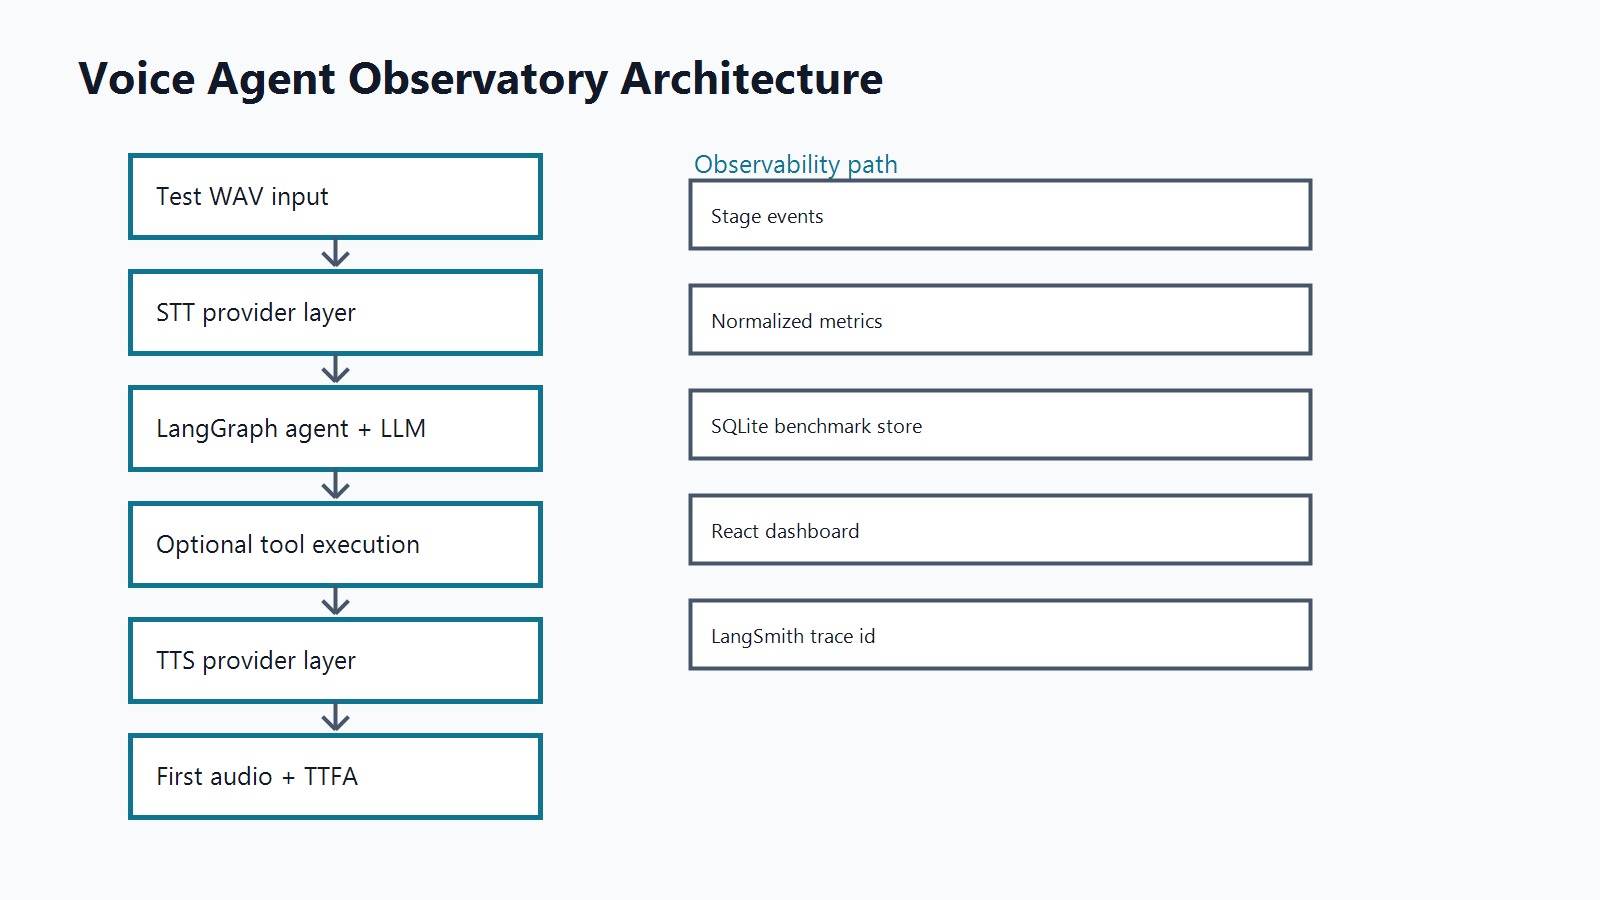
\includegraphics[width=0.92\textwidth]{figures/architecture.png}
  \caption{Architecture overview. The benchmark executes a fixed WAV through
  provider layers, LangGraph, optional tools, TTS, storage, dashboard, and
  LangSmith observability.}
\end{figure}

\subsection{Component Responsibilities}

\begin{itemize}
  \item \textbf{Frontend}: React/Vite dashboard for test cases, pipeline
  configuration, live benchmark events, result detail, model comparison,
  reliability, and concurrency views.
  \item \textbf{FastAPI backend}: REST and WebSocket API, provider availability,
  benchmark run orchestration, exports, and concurrency tests.
  \item \textbf{Pipeline runner}: single timing authority for INPUT\_END,
  STT, LangGraph/LLM, tools, TTS, FIRST\_AUDIO, and final persistence.
  \item \textbf{Provider layer}: adapter factories for STT and TTS using
  allowlisted provider:model[:voice] specifications.
  \item \textbf{Storage}: SQLite rows plus JSON artifacts under
  \texttt{docs/benchmark-results/}.
  \item \textbf{Observability}: live WebSocket events, dashboard waterfalls,
  stored stage events, and optional LangSmith traces.
\end{itemize}

\subsection{Data, Control, and Observability Flow}

The control path starts in the dashboard, travels through the API request into
\texttt{PipelineConfig}, resolves adapters through factories, executes the
pipeline, and writes a run result. The observability path is parallel: each
stage emits normalized events, which feed the live UI, SQLite storage, raw JSON
artifacts, and LangSmith metadata when tracing is enabled.

\section{Phase 3 - Model Plug-in Architecture}

The final implementation supports real model selection through a provider
registry rather than cosmetic dropdowns. STT and TTS choices are represented as
\texttt{provider:model[:voice]} specs. Unknown models are rejected by allowlists,
and unconfigured providers are marked unavailable rather than silently mapped to
another provider.

\begin{figure}[H]
  \centering
  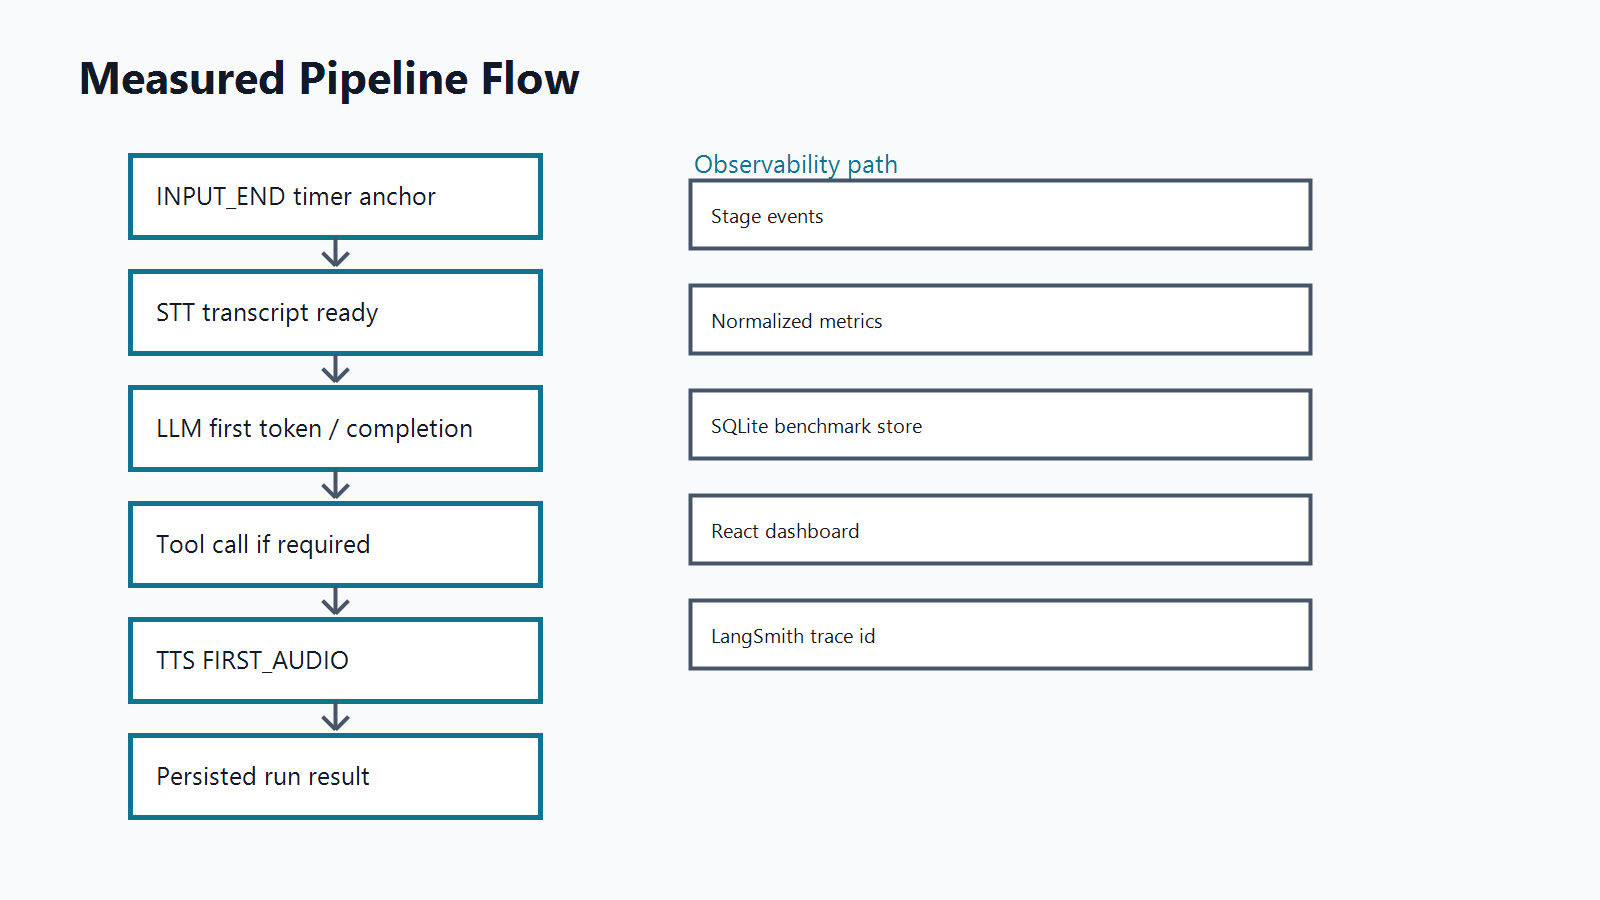
\includegraphics[width=0.92\textwidth]{figures/pipeline.png}
  \caption{Measured pipeline flow. TTFA is anchored at INPUT\_END and stops at
  the first actual audio bytes emitted by TTS.}
\end{figure}

\subsection{Implemented Providers}

\begin{longtable}{p{0.18\textwidth}p{0.22\textwidth}p{0.42\textwidth}p{0.11\textwidth}}
\toprule
Stage & Provider & Models & Status \\
\midrule
STT & Deepgram & nova-2, nova-3, hosted whisper-large & Verified \\
STT & ElevenLabs & scribe\_v1 & Verified earlier; quota/auth limited later \\
TTS & Deepgram & aura-2-thalia-en, aura-2-andromeda-en & Verified \\
TTS & ElevenLabs & eleven\_turbo\_v2\_5, eleven\_multilingual\_v2, eleven\_flash\_v2\_5 & Verified earlier; quota limited later \\
TTS & OpenAI & tts-1 & NOT\_CONFIGURED; not faked \\
LLM & OpenRouter & configured OpenRouter chat model, including gpt-4.1-mini in final reports & Verified \\
\bottomrule
\end{longtable}

The complete pipeline configuration is stored with every run through fields such
as \texttt{stt\_spec}, \texttt{llm\_spec}, \texttt{tts\_spec},
\texttt{tts\_voice\_id}, trace ID, events, and timings. Secrets remain server-side
in environment variables and are not exposed to frontend JavaScript.

\section{Phase 4 - Benchmark Execution}

The benchmark workload is the six provided WAV recordings imported into
\texttt{data/test\_cases/}. The repository metadata identifies no-tool cases,
tool cases, and noisy cases. The runner preserves the same audio bytes across
comparisons.

\begin{longtable}{p{0.16\textwidth}p{0.52\textwidth}p{0.14\textwidth}p{0.12\textwidth}}
\toprule
Case & Description & Expected tools & Noise \\
\midrule
TC01 & Direct spoken query & 0 & none \\
TC02 & Direct spoken query & 0 & none \\
TC03 & Weather query & 1 & none \\
TC04 & Web search query & 1 & none \\
TC05 & Noisy knowledge question & 0 & environmental \\
TC06 & Noisy direct query & 0 & environmental \\
\bottomrule
\end{longtable}

The final repository contains 415 benchmark JSON artifacts. Reports document
experiment IDs including \texttt{EXP-2026-00003}, \texttt{EXP-MULTI-*}, and
\texttt{EXP-FINAL-*}. Some named final experiment aggregate files are not present
as standalone \texttt{EXP-FINAL*.json} files; the raw per-run artifacts remain
present under \texttt{docs/benchmark-results/}.

\section{Phase 5 - Latency Measurement}

The backend records stage timestamps with a monotonic clock anchored at the end
of user audio. The main metrics are:

\begin{itemize}
  \item STT latency: provider call start to transcript ready.
  \item LLM TTFT and completion: LangGraph agent start to first token and final response.
  \item Tool latency: actual tool body execution time.
  \item TTS first-audio latency: TTS start to first emitted audio chunk.
  \item TTFA: INPUT\_END to FIRST\_AUDIO.
  \item Total response latency: INPUT\_END to TTS completion.
\end{itemize}

\begin{figure}[H]
  \centering
  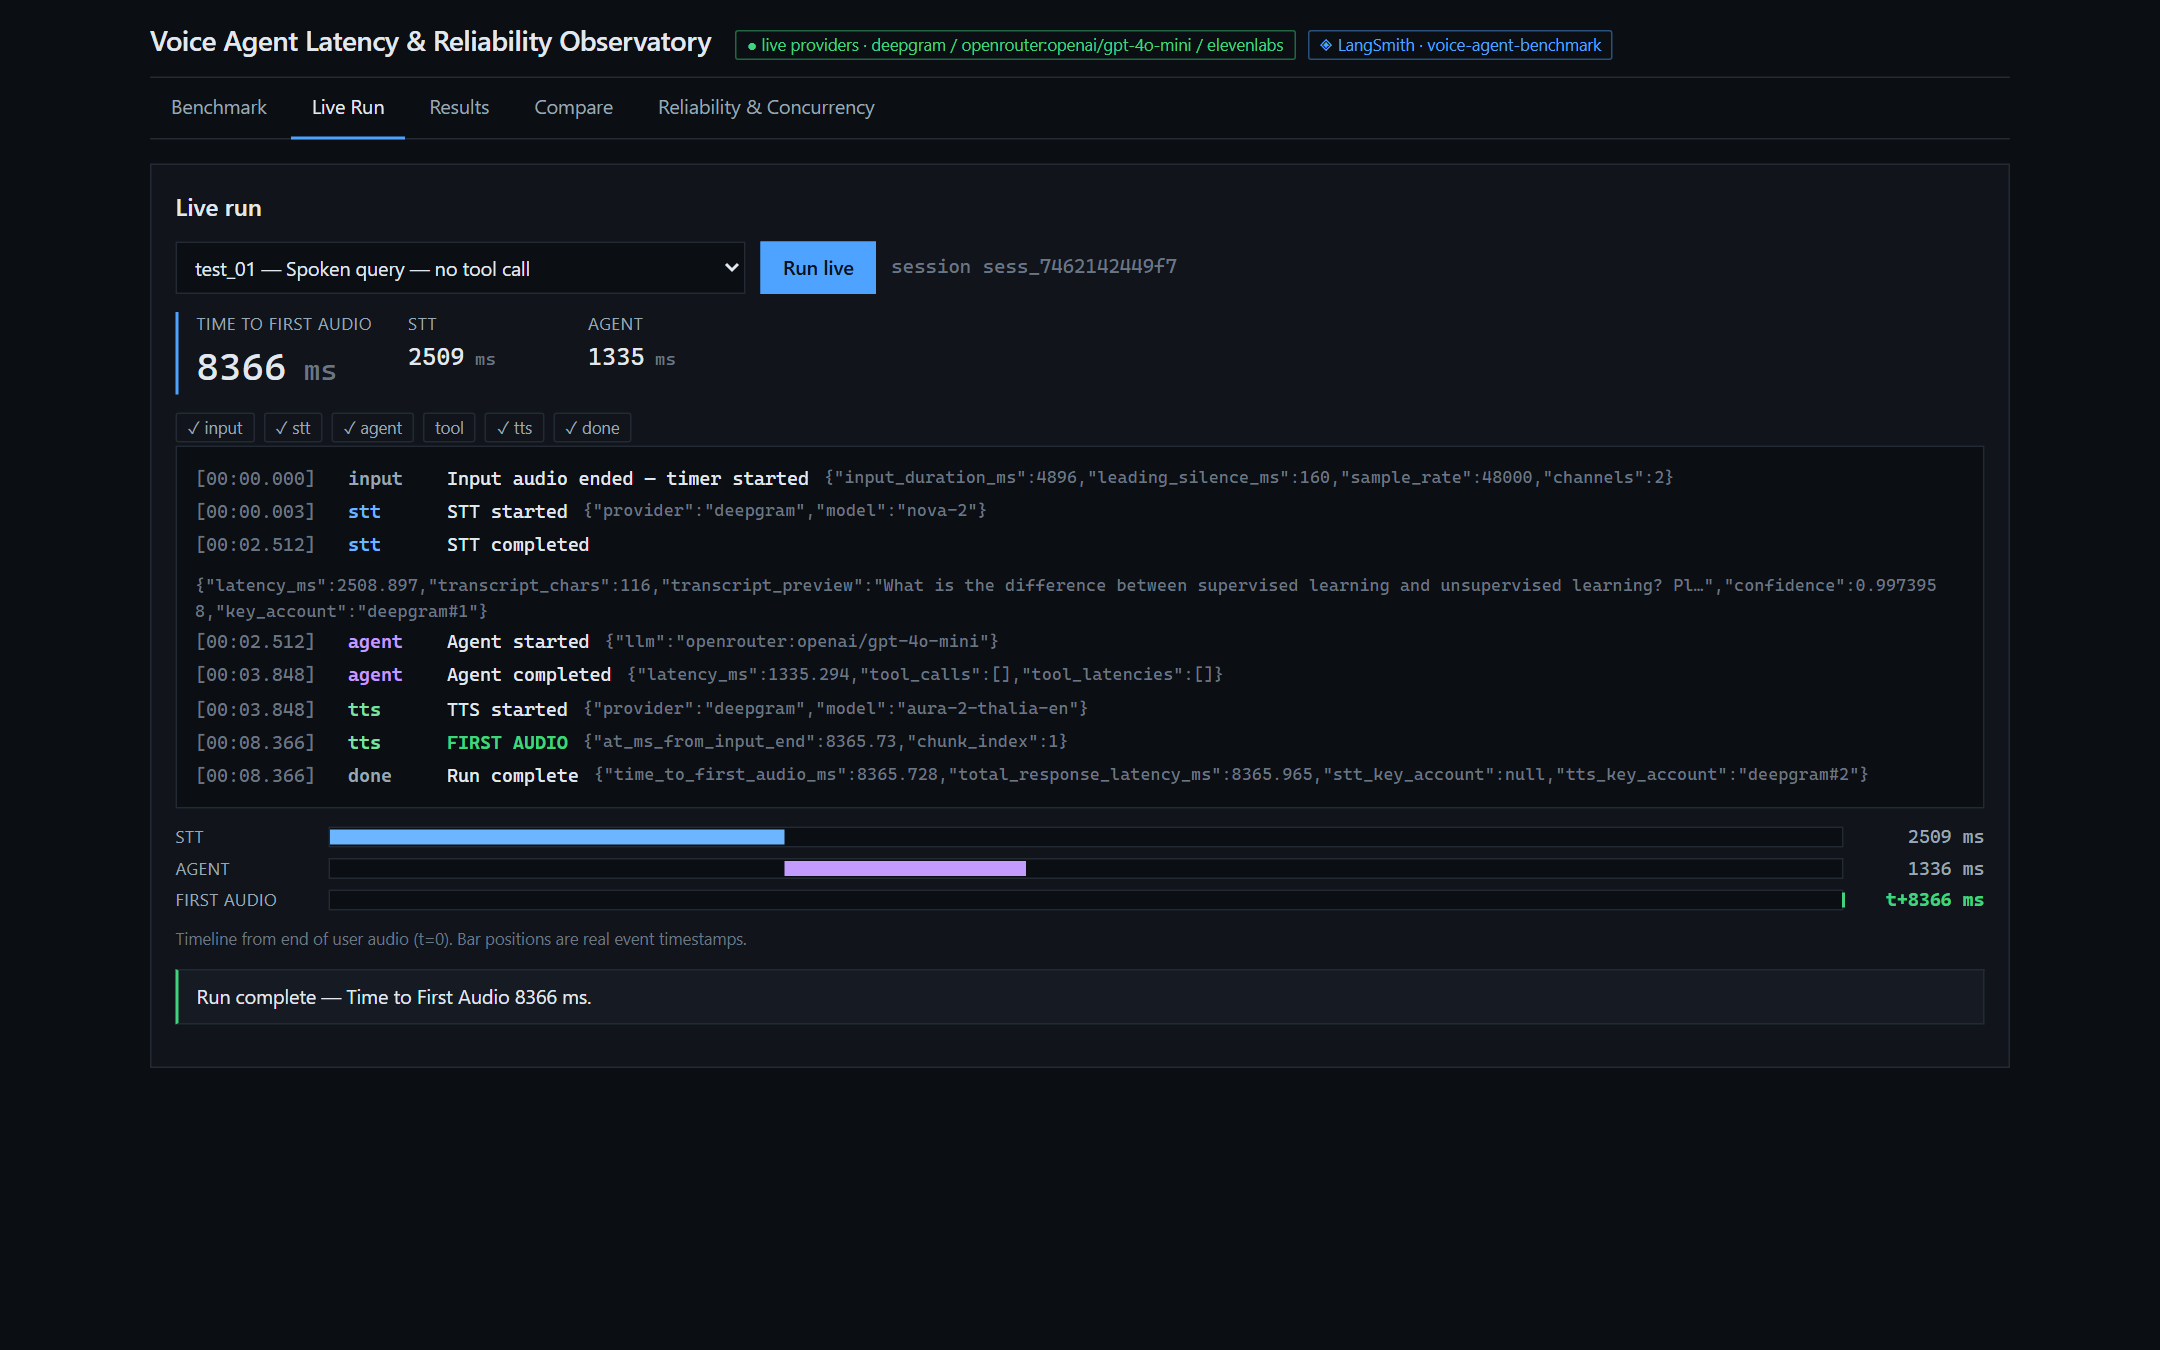
\includegraphics[width=0.92\textwidth]{figures/latency-waterfall.png}
  \caption{Latency waterfall screenshot. The UI visualizes stored stage events,
  including the FIRST AUDIO boundary used for TTFA.}
\end{figure}

Providers that return a single buffered audio response are labeled
\texttt{BUFFERED\_RESPONSE}; the system does not pretend that these providers
streamed first audio before completion.

\section{Phase 6 - Compare Models}

The final multi-model test report records same-input STT, same-text TTS, and
full pipeline comparisons. Results below are copied from repository reports and
are not generalized beyond the measured runs.

\begin{longtable}{p{0.25\textwidth}p{0.18\textwidth}p{0.18\textwidth}p{0.14\textwidth}p{0.1\textwidth}}
\toprule
STT & LLM & TTS & Test case & TTFA \\
\midrule
Deepgram nova-2 & gpt-4.1-mini & Aura Thalia & TC01 & 9,582 ms \\
Deepgram nova-3 & gpt-4.1-mini & Aura Thalia & TC01 & 8,811 ms \\
Deepgram whisper-large & gpt-4.1-mini & Aura Thalia & TC05 & 8,910 ms \\
Deepgram nova-3 & gpt-4.1-mini & Aura Andromeda & TC01 & 7,474 ms \\
Deepgram nova-2 & gpt-4.1-mini & ElevenLabs turbo & TC01 & failed at TTS quota \\
\bottomrule
\end{longtable}

\begin{figure}[H]
  \centering
  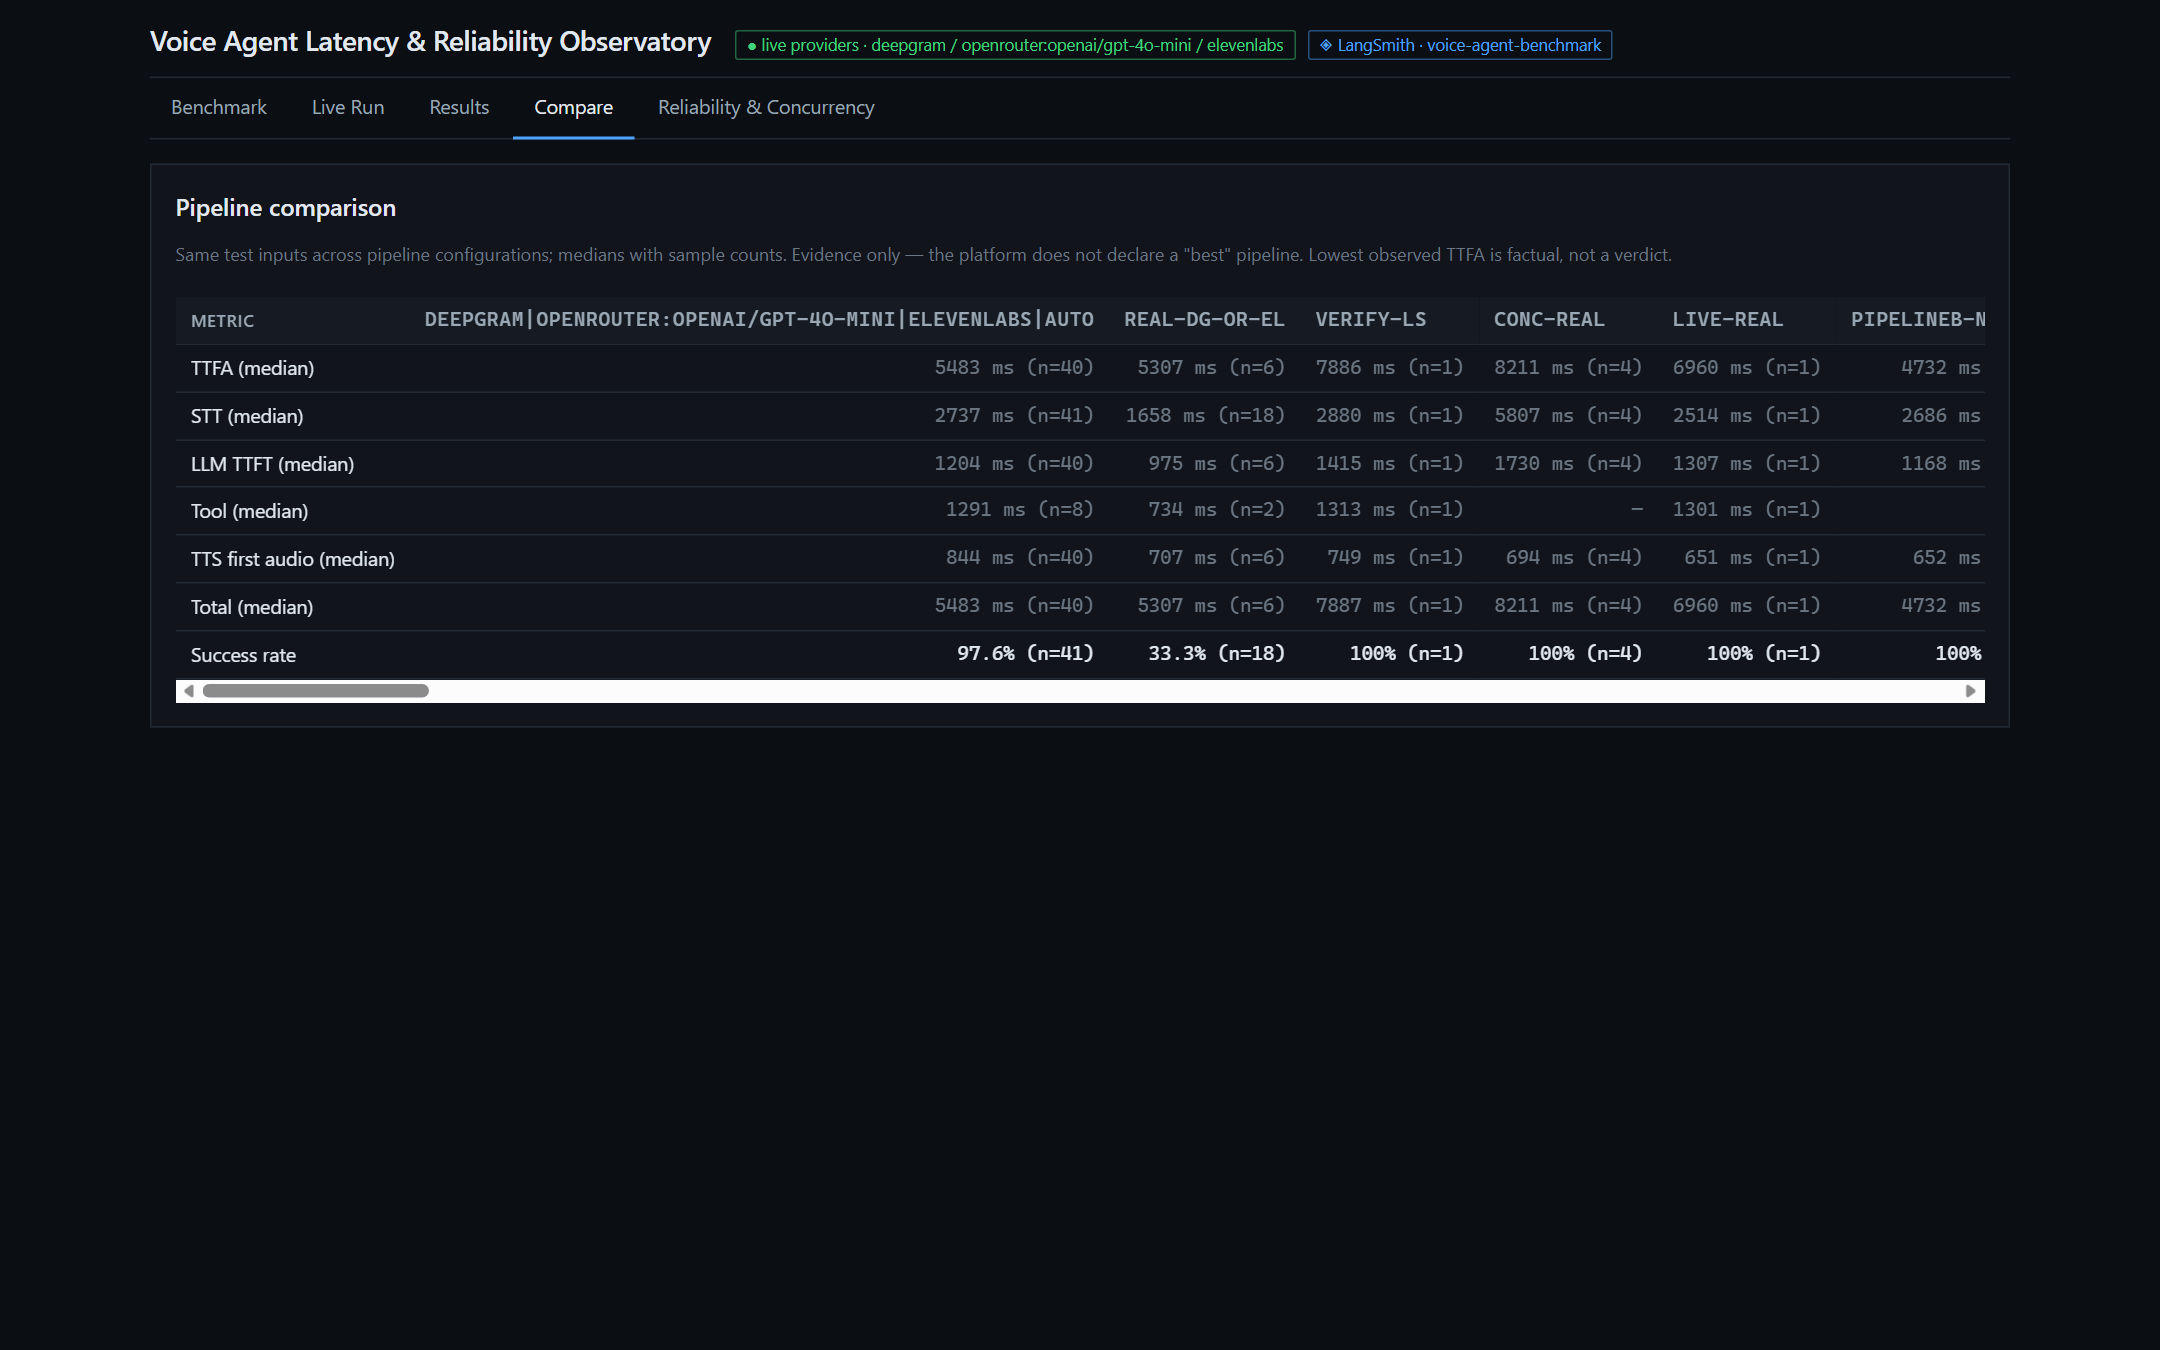
\includegraphics[width=0.92\textwidth]{figures/screenshots/model-comparison.png}
  \caption{Model comparison dashboard. Comparisons are based on stored runs and
  show counts and stage timing rather than declaring a universal best model.}
\end{figure}

The earlier \texttt{EXP-2026-00003} experiment compared OpenRouter models with a
shared Deepgram STT and ElevenLabs TTS setup: gpt-4.1-mini had median TTFA
6,093 ms over 12 runs, while gemini-3.8-flash had median TTFA 6,945 ms over
12 runs. The report also records that gemini over-called the weather tool on
TC03, which increased latency.

\section{Phase 7 - Reliability Testing}

Reliability work covers provider timeouts, quota failures, invalid audio,
tool behavior, LLM failures, TTS failures, and safe error visibility. The system
records \texttt{failure\_stage}, \texttt{error\_type}, safe error detail, provider
specs, and timestamps. Failures are retained as benchmark data instead of being
deleted from aggregates.

\begin{figure}[H]
  \centering
  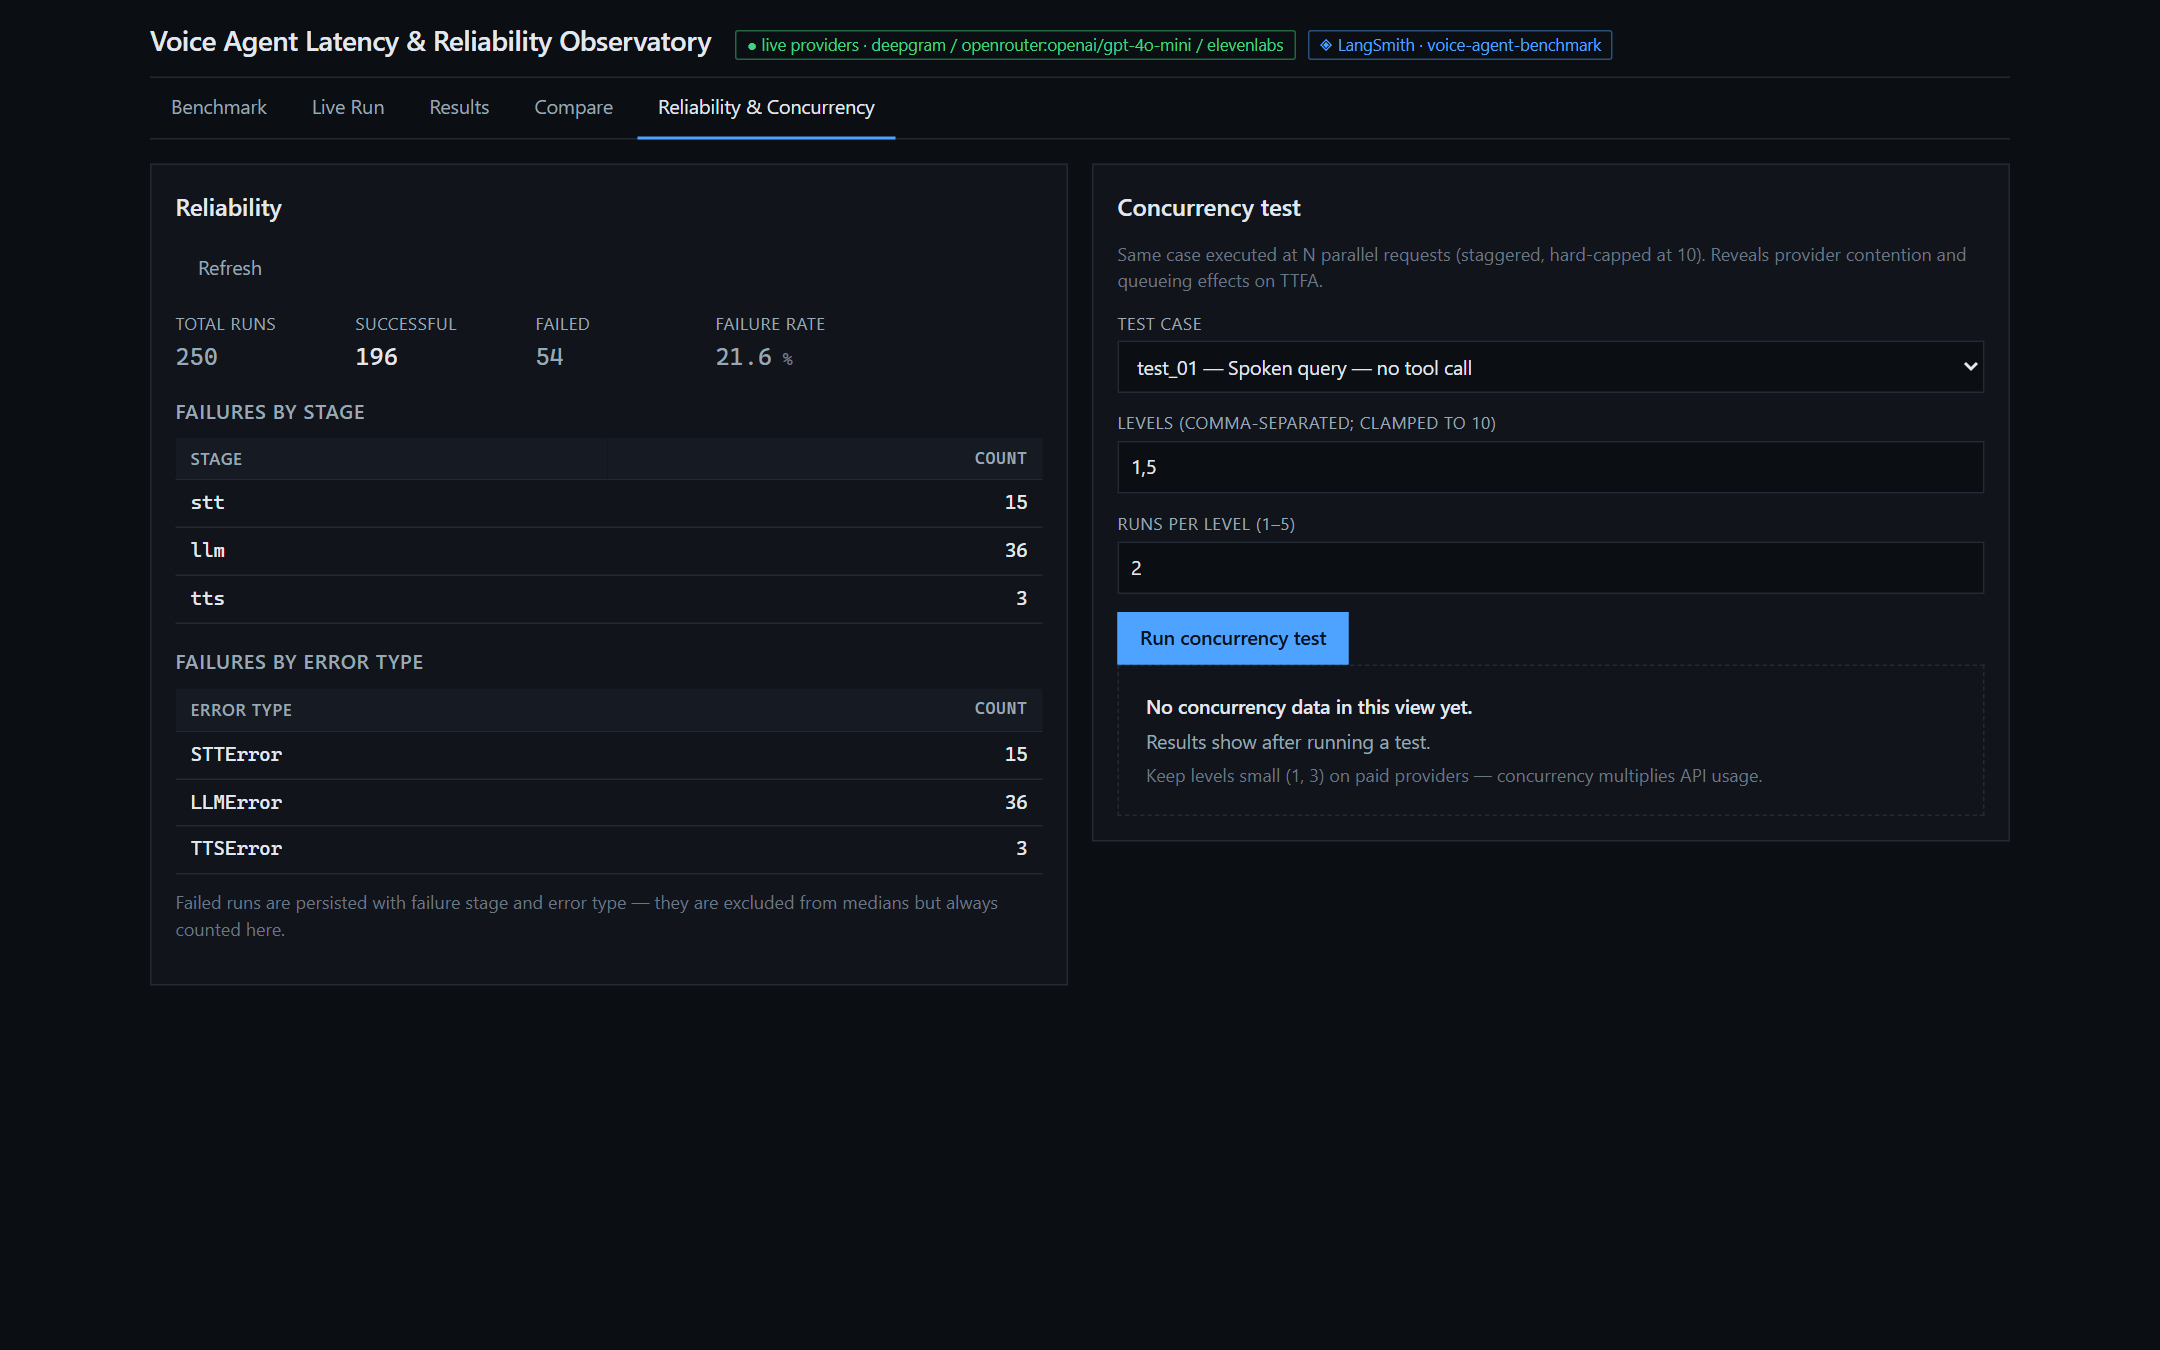
\includegraphics[width=0.92\textwidth]{figures/screenshots/reliability-summary.png}
  \caption{Reliability dashboard. Failure counts are stage-tagged so the operator
  can see whether failures came from STT, LLM, tools, TTS, input validation, or
  provider configuration.}
\end{figure}

Known retained failures include retired model IDs, provider credit limits,
quota-exceeded ElevenLabs TTS calls, and hosted whisper cold starts. These are
documented as limitations and surfaced in the UI.

\section{Phase 8 - Basic Concurrency Test}

The repository documents concurrency testing at levels 1 and 5 with the real
paid stack and level 1/5 mock validation in the final audit. Level 10 is
available and capped in the UI/backend, but the final real-stack report does not
claim level 10 was exercised because quota preservation mattered.

\begin{longtable}{p{0.18\textwidth}p{0.18\textwidth}p{0.22\textwidth}p{0.22\textwidth}}
\toprule
Level & Success & TTFA median & Throughput \\
\midrule
1 real stack & 2/2 & 5,913 ms & 0.30 rps \\
5 real stack & 10/10 & 6,896 ms & 1.16 rps \\
10 real stack & Not claimed & \na & \na \\
\bottomrule
\end{longtable}

\begin{figure}[H]
  \centering
  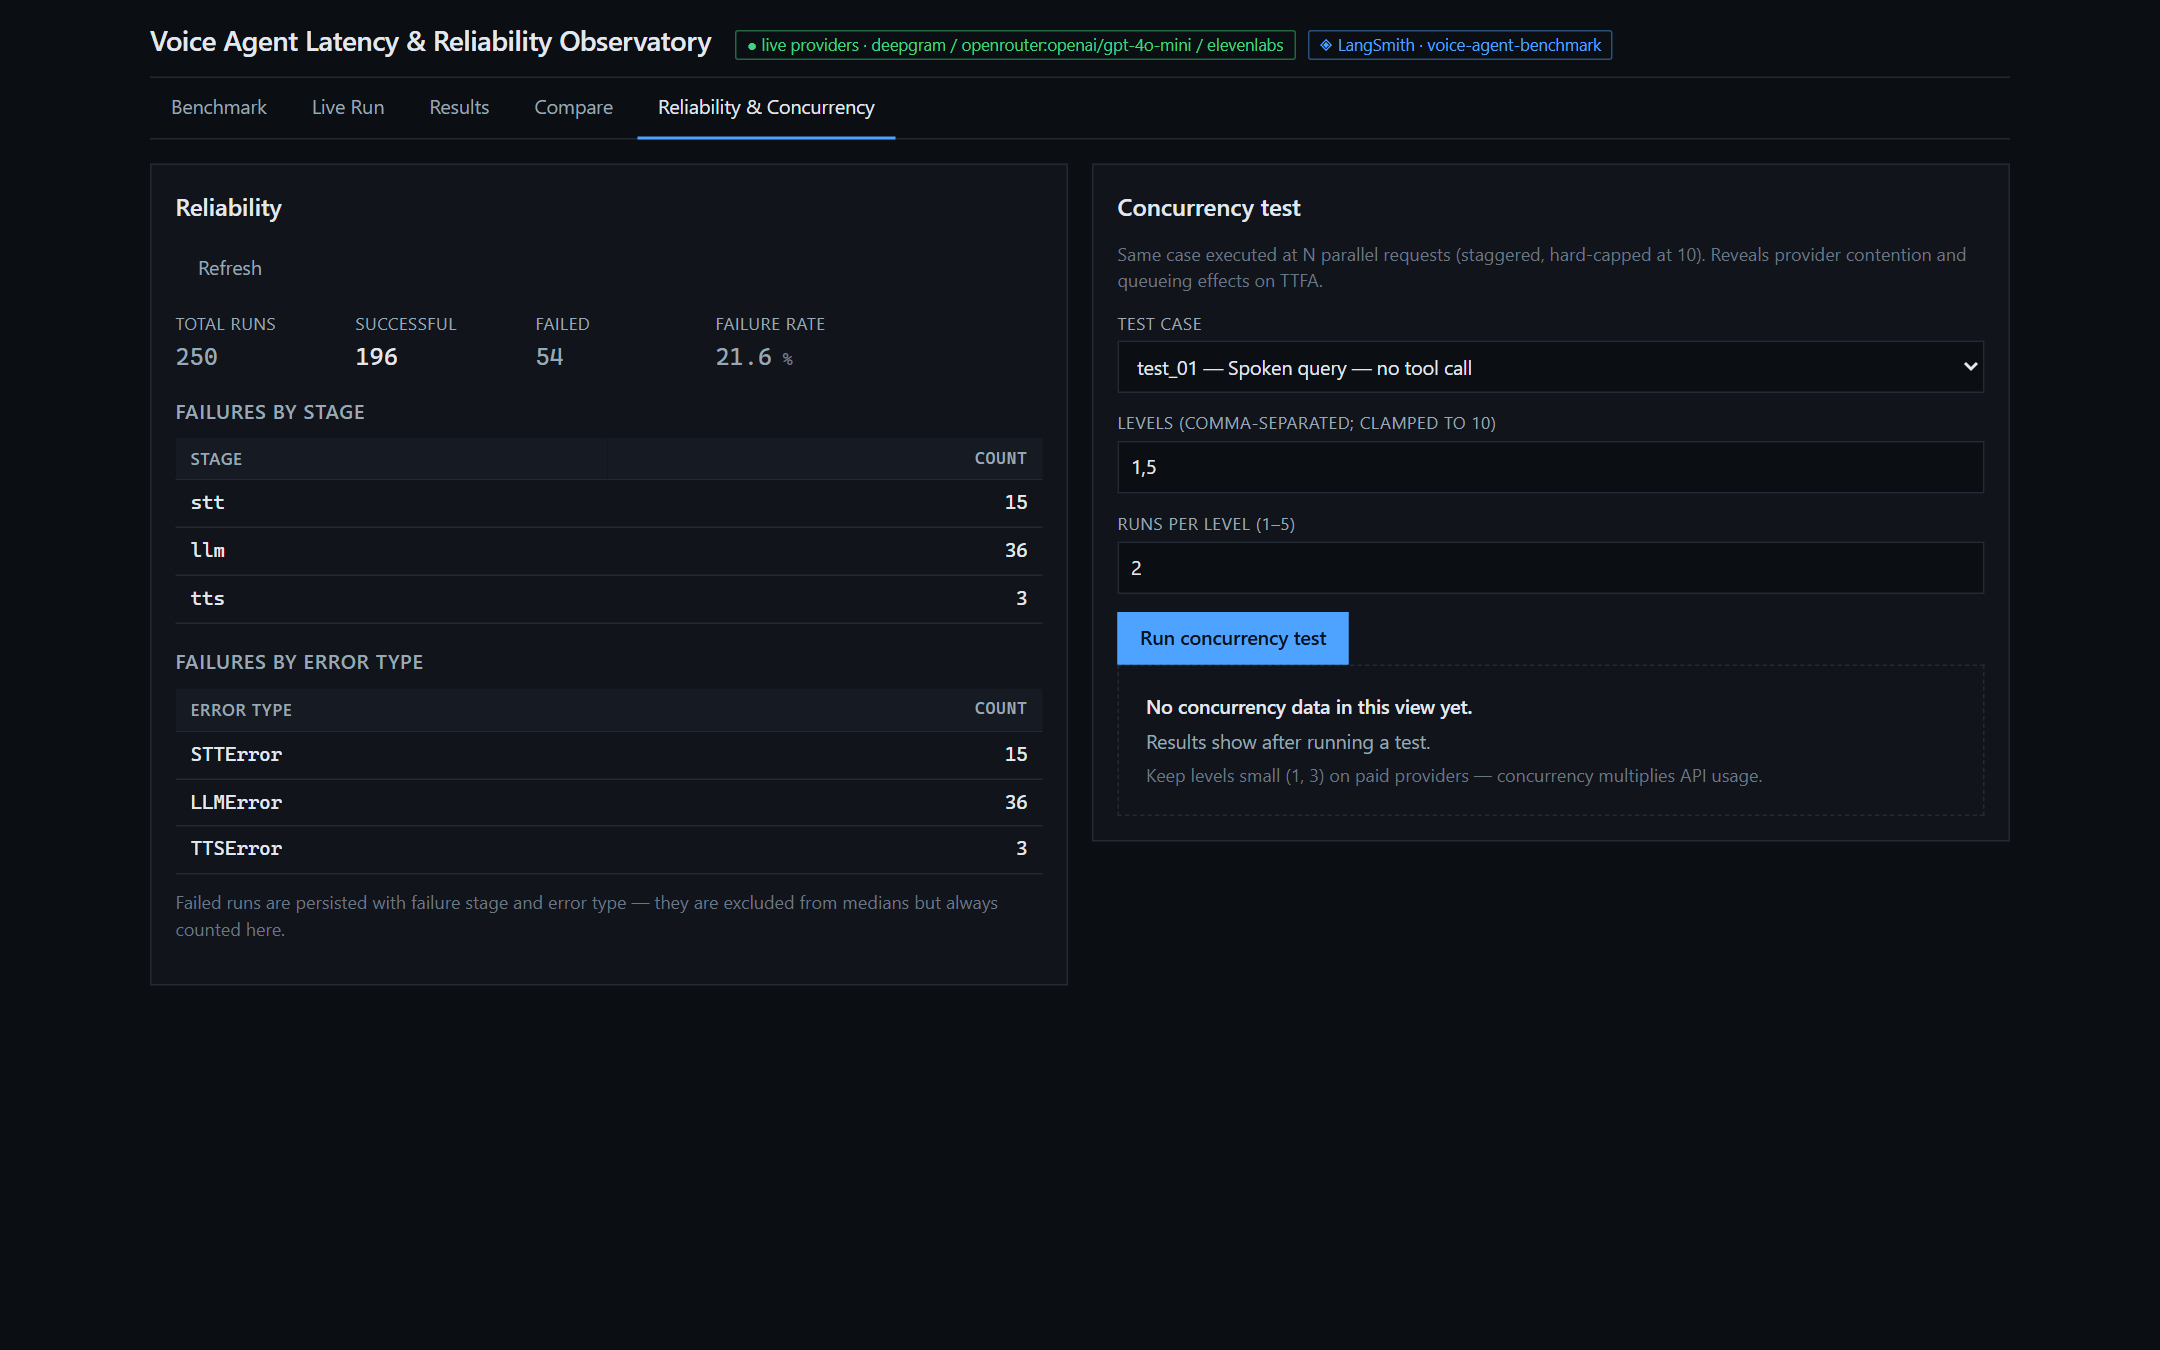
\includegraphics[width=0.92\textwidth]{figures/screenshots/concurrency-panel.png}
  \caption{Concurrency panel. The UI exposes concurrency controls while the
  backend clamps limits to protect provider quotas.}
\end{figure}

\section{Phase 9 - Frontend / Observability Dashboard}

The dashboard is an engineering console: dense tables, provider selectors,
availability states, live event streams, waterfall timing, run detail, comparison,
failure, trace, and concurrency views.

\begin{figure}[H]
  \centering
  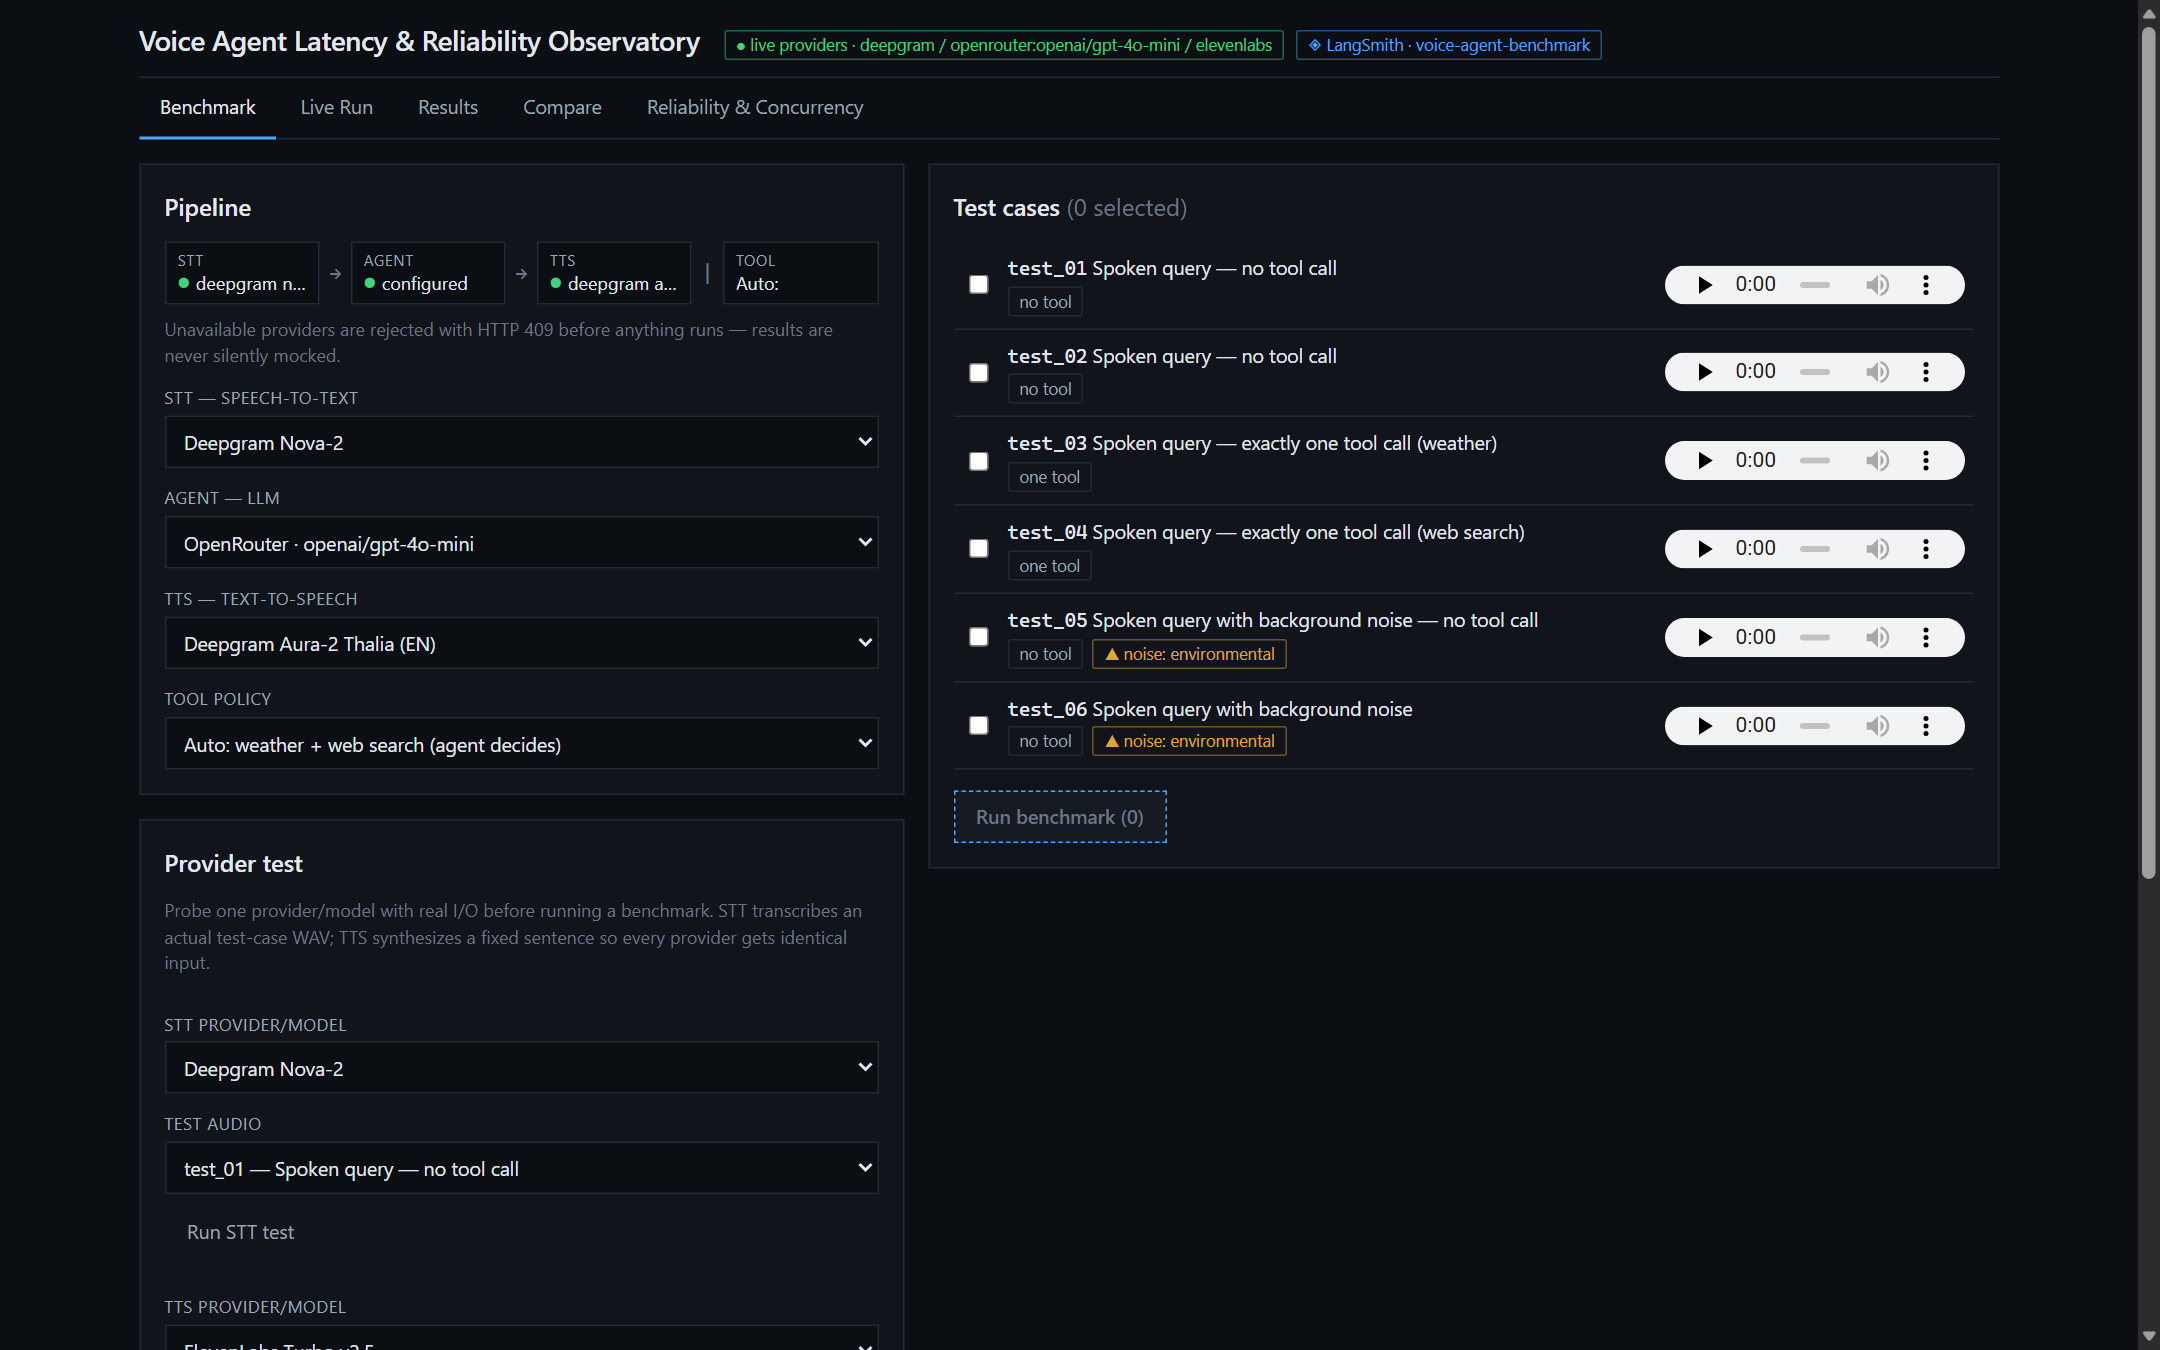
\includegraphics[width=0.92\textwidth]{figures/screenshots/dashboard-overview.png}
  \caption{Dashboard overview. The first screen emphasizes operational status,
  current metrics, and recent benchmark evidence.}
\end{figure}

\begin{figure}[H]
  \centering
  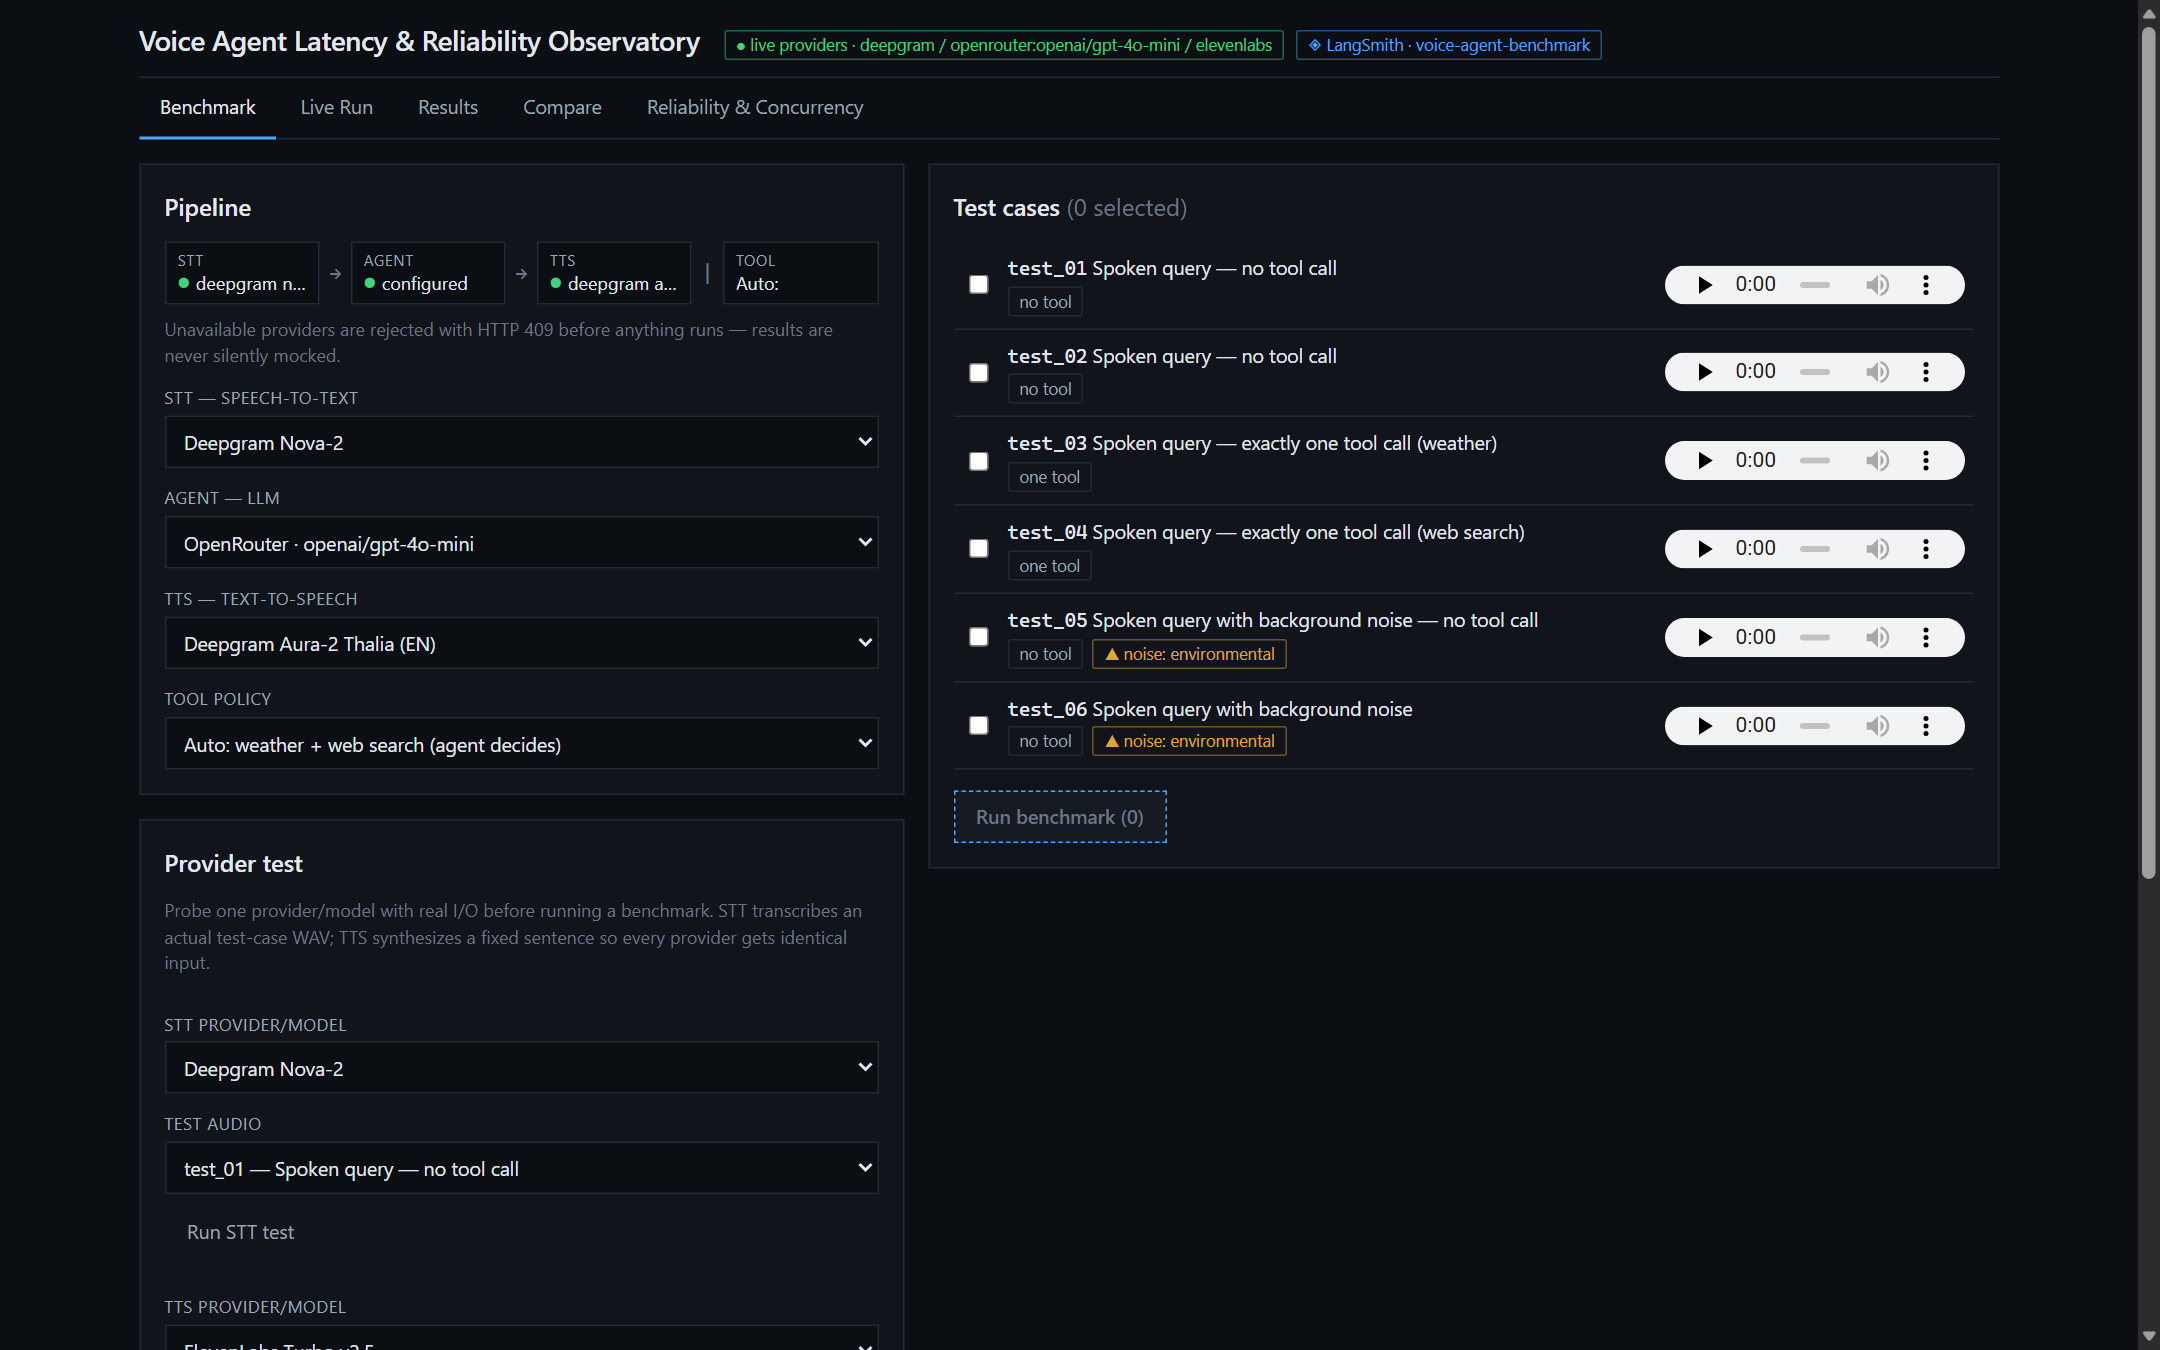
\includegraphics[width=0.92\textwidth]{figures/screenshots/pipeline-configuration.png}
  \caption{Pipeline configuration. Provider/model choices are exposed through
  the UI and submitted to the backend as executable pipeline specs.}
\end{figure}

\section{Phase 10 - Final Summary}

The repository contains a working voice-agent observatory with configurable STT,
LLM, and TTS stages; event-level instrumentation; TTFA measurement from
INPUT\_END to FIRST\_AUDIO; LangGraph execution; optional tool timing; LangSmith
trace IDs; SQLite persistence; model comparison; reliability and concurrency
views; security controls; and extensive audit documentation.

The main limitations are also explicit: ElevenLabs free-tier quota exhausted
after earlier successful verification, OpenAI TTS not configured, hosted
whisper cold starts, buffered rather than streaming first-audio semantics for
current working TTS providers, no auth for the local dashboard, and no claimed
real-stack level-10 concurrency run.

\section{Phase 11 - Source Code}

Repository URL:
\url{https://github.com/Sudesh-chandra/VoiceAgentDashboard.git}

\subsection{Repository Structure}

\begin{itemize}
  \item \texttt{backend/}: FastAPI API, pipeline runner, provider adapters,
  LangGraph agent, storage, tests, and scripts.
  \item \texttt{frontend/}: React/Vite dashboard.
  \item \texttt{data/test\_cases/}: six imported WAV test cases and metadata.
  \item \texttt{docs/}: architecture, assumptions, model reports, audit reports,
  benchmark artifacts, and this technical report.
  \item \texttt{screenshots/}: captured dashboard evidence.
  \item \texttt{AI\_USAGE.md}: AI assistance and engineering decision log.
\end{itemize}

\subsection{Reproduction Summary}

Set up environment variables from \texttt{.env.example}; do not commit
\texttt{.env}. Install backend and frontend dependencies. Run backend tests with
\texttt{MOCK\_MODE=true}; start the FastAPI server; start the Vite frontend; use
the dashboard or \texttt{backend/benchmark/run\_matrix.py} for benchmark runs.

\bibliographystyle{plain}
\bibliography{references}

\end{document}
